\documentclass[]{jarticle}
\usepackage{jtwocolumn,jscescnf}
\usepackage[dvipdfmx]{graphicx}
\usepackage{url}
\usepackage[caption=false]{subfig}
\urlstyle{rm}

\usepackage{amsmath,times,txfonts,bm}
\usepackage[ipaex]{pxchfon}          % 和文: IPAex 明朝・ゴシック
\usepackage[scaled=0.92]{helvet}     % 見出しの欧文: Helvetica 系
\makeatletter                        % 見出しをゴシック・サンセリフの太字に
\def\section{\@startsection {section}{1}{\z@}{2.5ex plus -.1ex minus -.1ex}{.001ex plus .1ex}{\reset@font\normalsize\gtfamily\sffamily\bfseries}}
\def\subsection{\@startsection{subsection}{1}{\z@}{3.25ex plus .1ex minus.1ex}{.1ex plus.1ex}{\reset@font\normalsize\gtfamily\sffamily\bfseries}}
\def\paragraph{\@startsection{paragraph}{4}{\z@}{.2ex plus.1ex minus.1ex}{-1em}{\reset@font\normalsize\gtfamily\sffamily\bfseries}}
\makeatother
\usepackage{booktabs}
\usepackage{algorithm}
\usepackage{algorithmic}
\usepackage{tikz}
\usetikzlibrary{shapes.geometric,arrows.meta,positioning,fit,backgrounds,calc}

% ---- spacing ----
\renewcommand{\baselinestretch}{0.97}
\setlength{\parskip}{0pt}

% ---- macros ----
\newcommand{\ten}[1]{\boldsymbol{#1}}
\newcommand{\dev}{\operatorname{dev}}
\newcommand{\bphi}{\boldsymbol{\phi}}
\newcommand{\bpsi}{\boldsymbol{\psi}}
\newcommand{\btheta}{\boldsymbol{\theta}}
\newcommand{\yobs}{\mathbf{y}_{\mathrm{obs}}}

% ***** 日本語タイトル *****
\title{
Hamilton 原理に基づく多菌種バイオフィルムモデルの Bayes 推定と\\
有限要素成長解析への組み込み
}
\endtitle{
Bayesian Calibration of a Hamilton-Principle Multi-Species Biofilm Model\\
and its Coupling into a Finite Element Growth Framework
}

\author{%
西岡佳祐（82519093）\thanks{慶應義塾大学 大学院 理工学研究科 開放環境科学専攻
(E-mail: keisuke58@keio.jp)}
，
村松眞由\thanks{慶應義塾大学 大学院 理工学研究科
(E-mail: muramatsu@mech.keio.ac.jp)}%
}
\endauthor{Keisuke Nishioka, Mayu Muramatsu}

\abstract{
A point model of a multi-species biofilm describes how the composition at one
material point evolves in time, but has no space; a continuum growth model
describes where a biofilm grows and what stresses it carries, but does not
distinguish species. Both follow from the extended Hamilton principle. First,
the 15 interaction coefficients of a five-species point model are estimated
with a two-phase, GPU-accelerated transitional Markov chain Monte Carlo
(TMCMC) method from in-vitro time courses under four conditions; the forward
model runs about 200 times faster than on the CPU, and the inferred
interactions predict the measured pH, which was not used in the calibration
($R^2=0.78$). Second, the growth kinematics $\mathbf F=\mathbf F_e\mathbf F_g$
with $\mathbf F_g=\alpha\mathbf I$ is implemented as an ANSYS user material,
verified against closed-form solutions, and coupled to the biofilm element of
the Institute of Continuum Mechanics (Leibniz University Hannover). Third, for
two species the point model runs at every Gauss point: the field sets the
amount of biofilm, the point model its composition. The stresses converge
under mesh refinement for the converted diffusion coefficient. The coupling is
one-way and verified, not validated.
}

\keywords{
Biofilm, Hamilton's Principle, TMCMC, Bayesian Inference, Growth Mechanics,
Finite Element Method, ANSYS User Material
}

\begin{document}

\renewcommand{\myaffil}{%
  {\footnotesize\bf 開放環境科学専攻 応用力学・計算力学専修}%
}

\maketitle
\thispagestyle{empty}

%%=================================================================
\section{研究背景・目的}
%%=================================================================

\subsection{出発点：Heine ら（2025）の実験観測}

Heine ら\cite{heine2025}は 5 菌種
（So: \textit{Streptococcus oralis}，An: \textit{Actinomyces naeslundii}，
Vei: \textit{Veillonella} spp.，Fn: \textit{Fusobacterium nucleatum}，
Pg: \textit{Porphyromonas gingivalis}）を用いた
口腔内バイオフィルムの in vitro 培養実験を行い，
共生（Commensal）・疾患型（Dysbiotic）$\times$
静置・HOBIC フローの 4 条件下で
Day 1/3/6/10/15/21 の菌種別体積分率を CLSM 定量化した．
疾患型 HOBIC 条件（DH）では
病原性 \textit{Pg}（W83 株）が後期に急増する
インプラント周囲炎型サージが観察されたが，
その力学機構---すなわち菌種間の相互促進・競合の強度と符号---は
実験データのみからは直接決定できない\cite{heine2025}．

\textbf{本研究の問い：}
Heine ら観測データから，5 菌種の相互作用を記述する
対称行列 $\mathbf{A}\in\mathbb{R}^{5\times5}$ の 15 パラメータを
定量的に推定できるか？またその事後分布から
Commensal/Dysbiotic 間でどのような力学的差異が浮かび上がるか？

\subsection{アプローチ}

Klempt ら\cite{klempt2026}は拡張 Hamilton 原理\cite{junker2021}の
停留条件 $\delta\mathcal{H}=0$ から，
菌種の体積分率 $\phi_i$ と生存率 $\psi_i$ が
相互作用行列 $\mathbf{A}$ を介して連動する材料点モデル（点モデル）を導出した．
一方 Klempt ら\cite{klempt2024}は同じ原理から，
バイオフィルムの量 $\phi$ と栄養 $c$ の場，成長変数 $\alpha$ を持つ
有限変形の成長モデルを示した．
前者は組成を扱うが空間を持たず，後者は空間と応力を扱うが菌種を区別しない．

本研究では，まず点モデルの相互作用を Heine ら\cite{heine2025}の
実験データから TMCMC\cite{ching2007} で推定し，
次に成長の運動学を，ハノーファー大学（LUH）連続体力学研究所で開発された
バイオフィルムの ANSYS 有限要素に組み込み，
最後に 2 菌種について点モデルを各 Gauss 点で動かして組成を求めた．

\subsection{研究目的と論文構成}

本報告の目的は以下の 3 点である：
\begin{enumerate}
  \item 5 菌種の点モデルの相互作用 15 成分を，
        2 段階 GPU-TMCMC で 4 条件の実験データから推定する（第 3--5 節）
  \item 成長の運動学 $\mathbf F_g=\alpha\mathbf I$ を ANSYS の材料ルーチンとして実装・検証し，
        バイオフィルムの有限要素に組み込む（第 6 節）
  \item 2 菌種について，場が量を，点モデルが組成を決める連成を行う（第 6 節）
\end{enumerate}
本報告は LUH 連続体力学研究所でのダブルディグリーの修士論文（2026 年 10 月提出）の内容に基づく．

%%=================================================================
\section{多種バイオフィルム連続体モデル}
%%=================================================================

\subsection{Klempt (2024) の単種有限変形モデル}\label{ssec:klempt24}

Klempt ら\cite{klempt2024}は Hamilton 原理に基づく
単種バイオフィルムの有限変形連続体モデルを提案した．
成長を弾性変形から分離する乗法分解
\begin{equation}
  \mathbf{F} = \mathbf{F}_e\mathbf{F}_g,\quad
  \mathbf{F}_g = \alpha\mathbf{I},\quad
  \det\mathbf{F}_g = \alpha^3
  \label{eq:multdecomp}
\end{equation}
（$\alpha$: 等方的成長変数）を採用し，
自由エネルギー密度（Eq.\,20）を
\begin{equation}
  \Psi = \phi\tfrac{\mu}{2}(I{:}\mathbf{C}^e-3)
       + \tfrac{\bar\beta}{2}|\nabla\phi|^2
       + \tfrac{\bar d}{2}|\nabla c|^2
       - \bar k_\alpha\alpha\phi
  \label{eq:psi_klempt}
\end{equation}
と定義した（$\mu$: せん断弾性率，$\bar\beta$: 界面正則化，$\bar k_\alpha$: 成長連成係数）．
Hamilton 原理の停留条件から得られる支配方程式（Eq.\,34--36）は
\begin{equation}
  \dot\phi = \beta\nabla^2\phi + k_\alpha\alpha + (\text{前線項}),\quad
  0 = d\nabla^2 c - g\phi,\quad
  \dot\alpha = k_\alpha\phi
  \label{eq:klempt34}
\end{equation}
であり，Cauchy 応力は
\begin{equation}
  \bm{\sigma} = \frac{\phi\mu}{\alpha^3}\dev(\mathbf{B}_e)+p\mathbf{I},\quad
  \mathbf{B}_e = \mathbf{F}_e\mathbf{F}_e^\top
  \label{eq:cauchy}
\end{equation}
と表される\cite{klempt2024}．
前線項はバイオフィルムの境界を栄養の勾配の方向へ動かす．
Klempt ら\cite{klempt2026}は同じ原理から下節の多菌種の点モデルを導出した．
本研究では成長の式（式\,\eqref{eq:klempt34} の第 3 式）を ANSYS の材料ルーチンに実装する（§6）．

\subsection{拡張 Hamilton 原理}\label{ssec:hamilton}

Klempt ら\cite{klempt2026}は Junker・Balzani\cite{junker2021}の
拡張 Hamilton 原理をバイオフィルム多種系に適用した．
Helmholtz 自由エネルギー $\mathcal{G}$，
体積制約 $\mathcal{C}$，
散逸ポテンシャル $\mathcal{D}$ を含む汎関数
\begin{equation}
  \mathcal{H} = \int_\tau (\mathcal{G} + \mathcal{C} + \mathcal{D})\,\mathrm{d}t
  \;\longrightarrow\; \text{stat.}
  \label{eq:hamilton}
\end{equation}
の停留条件 $\delta\mathcal{H}=0$ を各状態変数に対して取ることで，
支配方程式が系統的に導出される．
この定式化は熱力学第 1・第 2 法則の充足を
変分原理の段階で保証する\cite{junker2021}．

散逸ポテンシャルは粘性係数 $\eta_i$ を用いて
\begin{equation}
  \mathcal{D} = \frac{1}{2}\dot{\bar{\bphi}}^\top
  \boldsymbol{\eta}\,\dot{\bar{\bphi}}
  + \frac{1}{2}\dot{\bphi}^\top
  \boldsymbol{\eta}\,\dot{\bphi}
  \label{eq:dissipation}
\end{equation}
と定義される\cite{klempt2026}．第 1 項が $\dot\phi_i$--$\dot\psi_i$ の
非線形連成散逸を，第 2 項がフルランク正則化を与える．

\subsection{状態変数と多種相互作用}

体積分率 $\phi_i \in [0,1]$ と生存率 $\psi_i \in [0,1]$ の積
\begin{equation}
  \bar{\phi}_i = \phi_i\psi_i
  \label{eq:living}
\end{equation}
が生存体積分率であり，菌種間相互作用を担う．
空隙分率 $\phi_0$ を含む体積拘束
\begin{equation}
  \sum_{l=0}^{n} \phi_l = 1
  \label{eq:constraint}
\end{equation}
をラグランジュ乗数 $\gamma$ で課す．

自由エネルギー密度は栄養素濃度 $c^*$，
対称相互作用行列 $\mathbf{A}\in\mathbb{R}^{n\times n}$ を用いて
\begin{equation}
  \mathcal{G} = -\tfrac{1}{2}c^*\,\bar{\bphi}^\top \mathbf{A}\,\bar{\bphi}
  \label{eq:free_energy}
\end{equation}
と表される．$A_{ij}=A_{ji}$ は変分導出から自動的に保証され，
上三角成分 15 個が推定対象パラメータ $\btheta\in\mathbb{R}^{15}$ を構成する
（式\,\eqref{eq:free_energy} の二次形式から対称性が直接従う）．
Heine ら実験では抗生物質 $\alpha^*=0$ のため，
抗生物質感受性行列 $\mathbf{B}$ は消える．



\subsection{支配方程式（$\delta\mathcal{H}=0$ から導出）}

式\,\eqref{eq:hamilton} の停留条件を
$\phi_i$，$\psi_i$，$\gamma$ に対して取ると以下の連立 ODE が導出される\cite{klempt2026}：

\paragraph{体積分率 ODE（$\delta\mathcal{H}/\delta\phi_i=0$）}
\begin{equation}
  0 = -c^*\psi_i(\mathbf{A}\bar{\bphi})_i
    + \eta_i\!\left(\dot\phi_i\psi_i^2
    + \bar\phi_i\dot\psi_i + \dot\phi_i\right) + \gamma
  \label{eq:phi}
\end{equation}

\paragraph{生存率 ODE（$\delta\mathcal{H}/\delta\psi_i=0$）}
\begin{equation}
  0 = -c^*\phi_i(\mathbf{A}\bar{\bphi})_i
    + \eta_i\!\left(\dot\psi_i\phi_i^2
    + \bar\phi_i\dot\phi_i\right) + \gamma
  \label{eq:psi_evol}
\end{equation}

\paragraph{空隙・制約方程式（$\delta\mathcal{H}/\delta\gamma=0$）}
\begin{equation}
  \dot\phi_0 = -\gamma,\qquad
  \sum_{l=0}^{n}\phi_l = 1.
  \label{eq:phi0}
\end{equation}
系全体は $(2n+2)=12$ 本の連立非線形代数方程式となり，
各時間ステップで Newton 法により解かれる（§\ref{ssec:newton}）．

\subsection{相互作用行列の生物学的解釈}

Heine ら\cite{heine2025}が実験的に確認した
5 菌種間の主要なクロストーク経路（So--An 共凝集，So--Vei 乳酸交換，So--Fn ギ酸共生，Vei$\to$Pg pH 上昇，Fn--Pg ペプチド供給）を確認している．
$A_{ij}>0$ は種 $j$ が種 $i$ の成長を促進（協調），
$A_{ij}<0$ は抑制（競合）を意味する．
本研究では 15 パラメータすべてを事前に拘束せず推定し，
事後分布からスパース構造が自然に出現するかを検証する．



%%=================================================================
\section{GPU 加速 TMCMC によるパラメータ推定}
%%=================================================================

\subsection{実験観測データ（Heine 2025\cite{heine2025}）}

TMCMC の観測データは Heine ら\cite{heine2025}の
\textit{in vitro} バイオフィルム実験に基づく（表\,\ref{tab:conditions}）．
観測は Day 1/3/6/10/15/21 の 6 時点，各条件 $N\geq8$ 反復であり，
Day\,1 を初期条件として固定し，Day\,3--21 の 5 時点を尤度評価に使用する．
CLSM で取得した菌種別体積分率 $\phi_i^{\rm obs}$ を目的変数とし，
各時点・菌種の不均一分散 $\sigma_{ik}=\mathrm{IQR}/1.35$ を
異分散 Gaussian 尤度\eqref{eq:likelihood}として組み込んだ．
これにより，観測数が少ない Fn/Pg（共生条件で $\sigma_i\approx0.005$）は
大きく制約され，観測ばらつきが大きい So/Vei（$\sigma_i\approx0.2$）は
緩く制約される，物理的に整合した重み付けが実現される\cite{heine2025}．

\begin{table}[tb]
  \begin{center}
    \caption{実験条件（Heine 2025）}
    \vspace{2mm}
    \begin{tabular}{cll}\hline
      条件 & 菌種構成 & 培養形式 \\\hline
      CS & 共生菌 & 静置 \\
      CH & 共生菌 & 流動 (HOBIC) \\
      DS & 疾患型 & 静置 \\
      DH & 疾患型 & 流動 (HOBIC) \\\hline
    \end{tabular}
    \label{tab:conditions}
  \end{center}
\end{table}

\subsection{尤度と事前分布}

Gaussian 尤度は
\begin{equation}
  p(\mathcal{D}|\btheta)=
  \prod_{k=1}^{N_t}\prod_{i=0}^{4}
  \frac{1}{\sqrt{2\pi}\,\sigma_{ik}}
  \exp\!\left(-\frac{(\phi_i(t_k;\btheta)-\phi_i^{\rm obs}(t_k))^2}{2\sigma_{ik}^2}\right)
  \label{eq:likelihood}
\end{equation}
と定義する．事前分布は独立一様分布
\begin{equation}
  p(\btheta) = \prod_{k=0}^{14}\frac{1}{u_k-l_k}\,\mathbf{1}_{[l_k,u_k]}(\theta_k)
  \label{eq:prior}
\end{equation}
であり，初期範囲 $[l_k,u_k]\approx[-1,1]$ を Phase\,1a の事後分位点で縮小する
（iteratively narrowed prior 法）．

\subsection{数値実装：Newton 法と JAX 並列化}\label{ssec:newton}

各時間ステップ $\Delta t=10^{-4}$（$N_t=2{,}500$ ステップ，$t_{\max}=0.25$，
実験 21 日に対応）で implicit Euler を適用する．
状態ベクトル $\mathbf{x}=(\phi_1,\ldots,\phi_5,\phi_0,\psi_1,\ldots,\psi_5,\gamma)^\top$
$\in\mathbb{R}^{12}$ に対する残差
\begin{equation}
  \mathbf{R}(\mathbf{x}^{n+1}) = \mathbf{0}
  \label{eq:residual}
\end{equation}
を Newton 法（Jacobian 解析的評価）で反復解する．
対数バリア $\Psi_{\rm bar}=-K_p\ln(\phi_i(1-\phi_i))$（$K_p=\eta_i\times10^{-4}$）を
加えて $\phi_i,\psi_i\in(0,1)$ のボックス制約を維持する\cite{klempt2026}．

JAX 実装では \texttt{jax.jit} で Newton ソルバを単一 XLA カーネルにコンパイルし，
$N_p$ 粒子を \texttt{jax.vmap} で GPU 上に並列展開する．DH 条件・$N_p=500$・9 ステージで，CPU（12 コア）の 21600\,s が GPU では 147\,s となった（約 200 倍）．
この設計により，CPU では $N_p/12$ シリアルバッチを要した計算が
GPU では 1 バッチで完了する．



%%=================================================================
\section{2 段階 GPU-TMCMC アルゴリズム}
%%=================================================================

\subsection{アルゴリズム概要}

15 次元パラメータ空間における事後多峰性を回避するため，
表\,\ref{tab:phases} に示す 2 段階推定戦略を採用した\cite{klempt2026}．
Phase\,1 では生存率 $\psi_i$ を Heine 実測の膜完全性データから固定し，
Jacobian 次元を $2n+2=12$ から $n+2=7$ に半減させて
$\mathbf{A}$ を高速に同定する．
Phase\,2 では $\psi_i$ を解放し，
Phase\,1 事後分布を $\mathbf{A}$ の情報事前分布として利用することで，
$\mathbf{A}$--$\psi_i$ 結合事後分布を取得する．

\begin{table}[tb]
  \begin{center}
    \caption{2 段階推定戦略}
    \vspace{2mm}
    \begin{tabular}{cll}\hline
      Phase & $\psi_i$ の扱い & 事前分布（$N_p$）\\\hline
      1a & 実験値固定 & 広 ($[-1,1]$)（1k） \\
      1b & 実験値固定 & 縮小・1a 事後（1k） \\
      2  & 自由変数 & 1b 事後・情報事前（10k）\\\hline
    \end{tabular}
    \label{tab:phases}
  \end{center}
\end{table}

\subsection{TMCMC の逐次焼き戻し}

TMCMC\cite{ching2007,wu2018}は事前分布 $p(\btheta)$ から
事後分布 $p(\btheta|\mathcal{D})$ へ，中間分布列
\begin{equation}
  p_m(\btheta)\propto p(\mathcal{D}|\btheta)^{\beta_m}\,p(\btheta),
  \quad 0=\beta_0<\beta_1<\cdots<\beta_M=1
  \label{eq:tempered}
\end{equation}
を段階的に構築する逐次 Monte Carlo 法である．
各ステージの逆温度 $\beta_{m+1}$ は，
重み $w_j^{(m)}=p(\mathcal{D}|\btheta_j^{(m)})^{\beta_{m+1}-\beta_m}$ の
変動係数
\begin{equation}
  \mathrm{CoV}[\{w_j^{(m)}\}] = \delta_{\rm target}
  \label{eq:cov_target}
\end{equation}
を満たすよう二分探索で決定する．
MH 変異の提案分布は加重共分散
\begin{equation}
  \hat{\boldsymbol{\Sigma}}^{(m)}
  = \sum_{j}\bar{w}_j^{(m)}
  (\btheta_j^{(m)}-\bar{\btheta}^{(m)})
  (\btheta_j^{(m)}-\bar{\btheta}^{(m)})^\top
  \label{eq:wcov}
\end{equation}
を用いた $\mathcal{N}(\btheta_j,\gamma^2\hat{\boldsymbol{\Sigma}}^{(m)})$ とし，
受理率が 5\% 未満なら $\gamma\leftarrow\gamma/2$，
40\% 超なら $\gamma\leftarrow1.5\gamma$ と適応調整する．

\subsection{アルゴリズム全体フロー}

アルゴリズム全体を Algorithm\,\ref{alg:tmcmc} に示す．

\begin{algorithm}[tb]
\caption{2段階 GPU 加速 TMCMC}
\label{alg:tmcmc}
\begin{algorithmic}[1]
\REQUIRE 観測 $\mathcal{D}$，$\psi_i^{\rm exp}(t_k)$，$N_p$，GPU
\ENSURE $\hat{\btheta}^{\rm MAP}$，事後サンプル，$\ln\hat{Z}$
\STATE \textbf{Phase\,1a}: $\psi_i\leftarrow\psi_i^{\rm exp}$，$[l_k,u_k]=[-1,1]$
\STATE $\{\btheta_j\}_{j=1}^{N_p}\sim p_0(\btheta)$；$\beta_0\leftarrow0$
\WHILE{$\beta_m<1$}
  \STATE bisection: $\mathrm{CoV}[\{w_j\}]=\delta_{\rm target}$
        $\to\beta_{m+1}$
  \STATE $w_j\leftarrow p(\mathcal{D}|\btheta_j)^{\beta_{m+1}-\beta_m}$
  \STATE 系統的リサンプリング $\propto w_j$
  \STATE $\hat{\boldsymbol{\Sigma}}^{(m)}$ を推定（式\,\eqref{eq:wcov}）
  \FOR{$k=1$ \TO $K$}
    \STATE \texttt{vmap}：全 $N_p$ ODE を GPU 並列積分
    \STATE MH 受理・棄却；$\gamma$ を適応調整
  \ENDFOR
\ENDWHILE
\STATE 1a 事後 $q_{0.01}$/$q_{0.99}$ から事前幅を縮小
\STATE \textbf{Phase\,1b}: 狭事前で再実行
      $\to\hat{\btheta}^{\rm MAP}_{\rm fix\text{-}\psi}$，$\ln\hat{Z}_1$
\STATE \textbf{Phase\,2}: $\psi_i$ 解放；$\btheta$ 事前 $\leftarrow$ 1b 事後
\STATE 拡張尤度：$\ln\mathcal{L}\mathrel{+}=
  -\sum_{k,i}(\psi_i-\psi_i^{\rm exp})^2/(2\sigma_\psi^2)$
\STATE lines 3--11 を $N_p=10{,}000$ で繰り返す
\RETURN $\hat{\btheta}^{\rm MAP}$，$\hat{\bpsi}^{\rm MAP}$，$\ln\hat{Z}_2$
\end{algorithmic}
\end{algorithm}

%%=================================================================
\section{推定結果}
%%=================================================================

\subsection{事後予測フィット}

図\,\ref{fig:fitting} に 4 条件すべての
事後予測を Heine の実測値と重ねて示す．
共生条件では \textit{So}/\textit{An} の増殖が再現され，
\textit{Pg} は固定せずに推定からほぼゼロとなった（CS）．
流れのある CH では \textit{So} が優勢となる様子が再現された．
疾患型では，DS の病原菌の遷移と，DH の \textit{Vei}/\textit{Pg} の非線形な増幅
（後期のサージ）が捉えられた\cite{heine2025}．
信用区間は CS から DH にかけて広がる．

\begin{figure*}[tb]
  \centering
  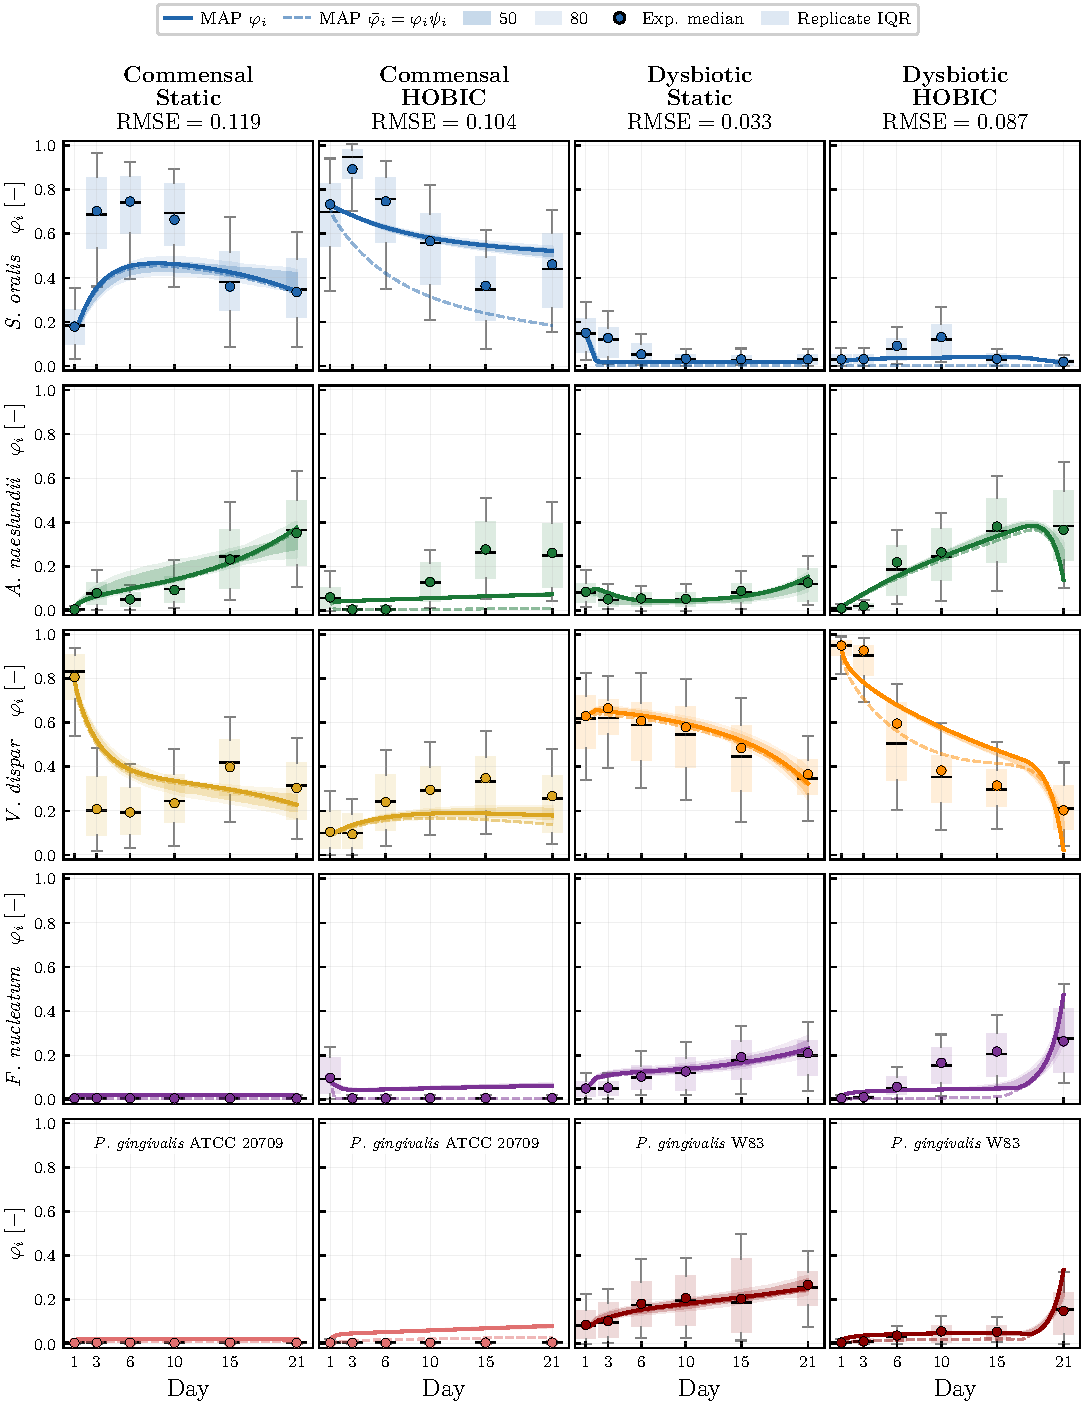
\includegraphics[width=0.72\textwidth]{heine_fits_4cond.pdf}
  \caption{\textbf{事後予測（4 条件 $\times$ 5 菌種，Phase\,2）．}
    列: CS/CH/DS/DH，行: So/An/Vei/Fn/Pg．実線: MAP，破線: 生存分率，
    帯: 50\%/80\% 信用区間，丸と箱: 実験の中央値と四分位範囲（$N=8$）．}
  \label{fig:fitting}
\end{figure*}

\subsection{相互作用行列 MAP 推定}

図\,\ref{fig:heatmap} に 4 条件の MAP 相互作用行列 $\mathbf{A}$ を示す．

共生条件（CS/CH）では \textit{So}--\textit{An} と \textit{So}--\textit{Vei} のブロックが主で，
\textit{Fn} と \textit{Pg} の行はほぼゼロとなった．
疾患型への移行で \textit{Vei}--\textit{Pg} と \textit{Fn}--\textit{Pg} の正の成分が強く現れた（§7.2）．

\begin{figure}[tb]
  \centering
  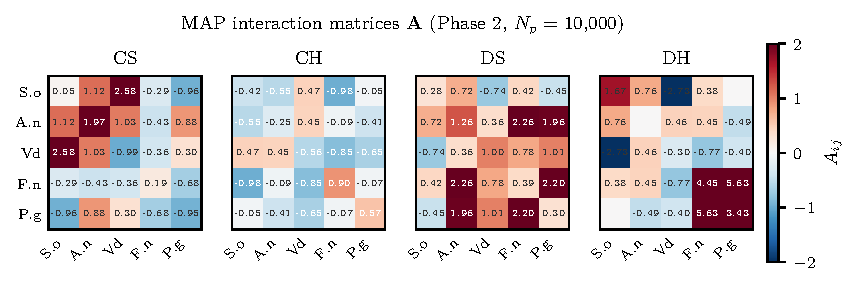
\includegraphics[width=\linewidth]{heine_heatmap_A_4cond.pdf}
  \caption{\textbf{MAP 相互作用行列 $\mathbf{A}$（4条件）．}
    赤: 協調（$A_{ij}>0$），青: 競合（$A_{ij}<0$）．
    CS/CH では Fn・Pg 行が事前制約なしにゼロへ収束する．}
  \label{fig:heatmap}
\end{figure}

\subsection{定量評価と pH による検証}

表\,\ref{tab:rmse} に Phase\,2（$\psi$ 自由，$N_p=10{,}000$）の RMSE を示す．
Phase\,1 からの増加は 0.03 以下であり，$\psi$ を解放しても相互作用の構造は保たれた．
DS が最もよく合い（RMSE 0.033），DH でも \textit{Pg} の $R^2=0.90$ を保った．

\begin{table}[tb]
  \begin{center}
    \caption{2 段階推定の RMSE（菌種平均）}
    \vspace{2mm}
    \begin{tabular}{ccc}\hline
      条件 & Phase\,1 & Phase\,2 \\\hline
      CS & 0.119 & 0.119 \\
      CH & 0.071 & 0.104 \\
      DS & 0.020 & 0.033 \\
      DH & 0.067 & 0.087 \\\hline
    \end{tabular}
    \label{tab:rmse}
  \end{center}
\end{table}

推定に使っていない HOBIC 条件の pH の時系列で，推定した $\mathbf A$ を検証した．
菌種の分率から pH を求める線形モデル（係数は交差検証で選んだ）を，
ODE が予測した分率に当てはめると，$R^2=0.778$（RMSE 0.126 pH 単位）となった．
$\mathbf A$ が群集の pH を決める要因を捉えていることを示す．

%%=================================================================
\section{バイオフィルム有限要素への組み込み\label{sec:fem_coupling}}
%%=================================================================

\subsection{枠組みと追加したもの}

このバイオフィルム要素は，力学を ANSYS で解き，
$\phi$ と $c$ の場を独自のルーチンで解く．
$\phi$ の Laplacian と勾配は，近くの積分点の値から 2 次の Taylor 展開を
重み付き最小二乗で当てはめて求める（Neighbored Element Method\cite{rudolf2025}）．
場は陽解法で更新され，力学とはサブステップごとに交互に進む．

私が追加したのは材料ルーチン（USERMAT）の部分である．
各 Gauss 点で場から $\phi$ を受け取り，成長の式
$\alpha_{n+1}=\alpha_n+k_\alpha\phi\,\Delta t$ を積分し，
$\mathbf F_g=\alpha\mathbf I$，$\mathbf F_e=\mathbf F\mathbf F_g^{-1}$ から
応力と接線剛性を返す．
2 菌種では，同じ Gauss 点で点モデル\cite{klempt2026}を動かし，
場が量 $\phi$ を，点モデルが組成 $\phi_1/(\phi_1+\phi_2)$ を決める（図\,\ref{fig:coupling}）．

\begin{figure*}[tb]
  \centering
  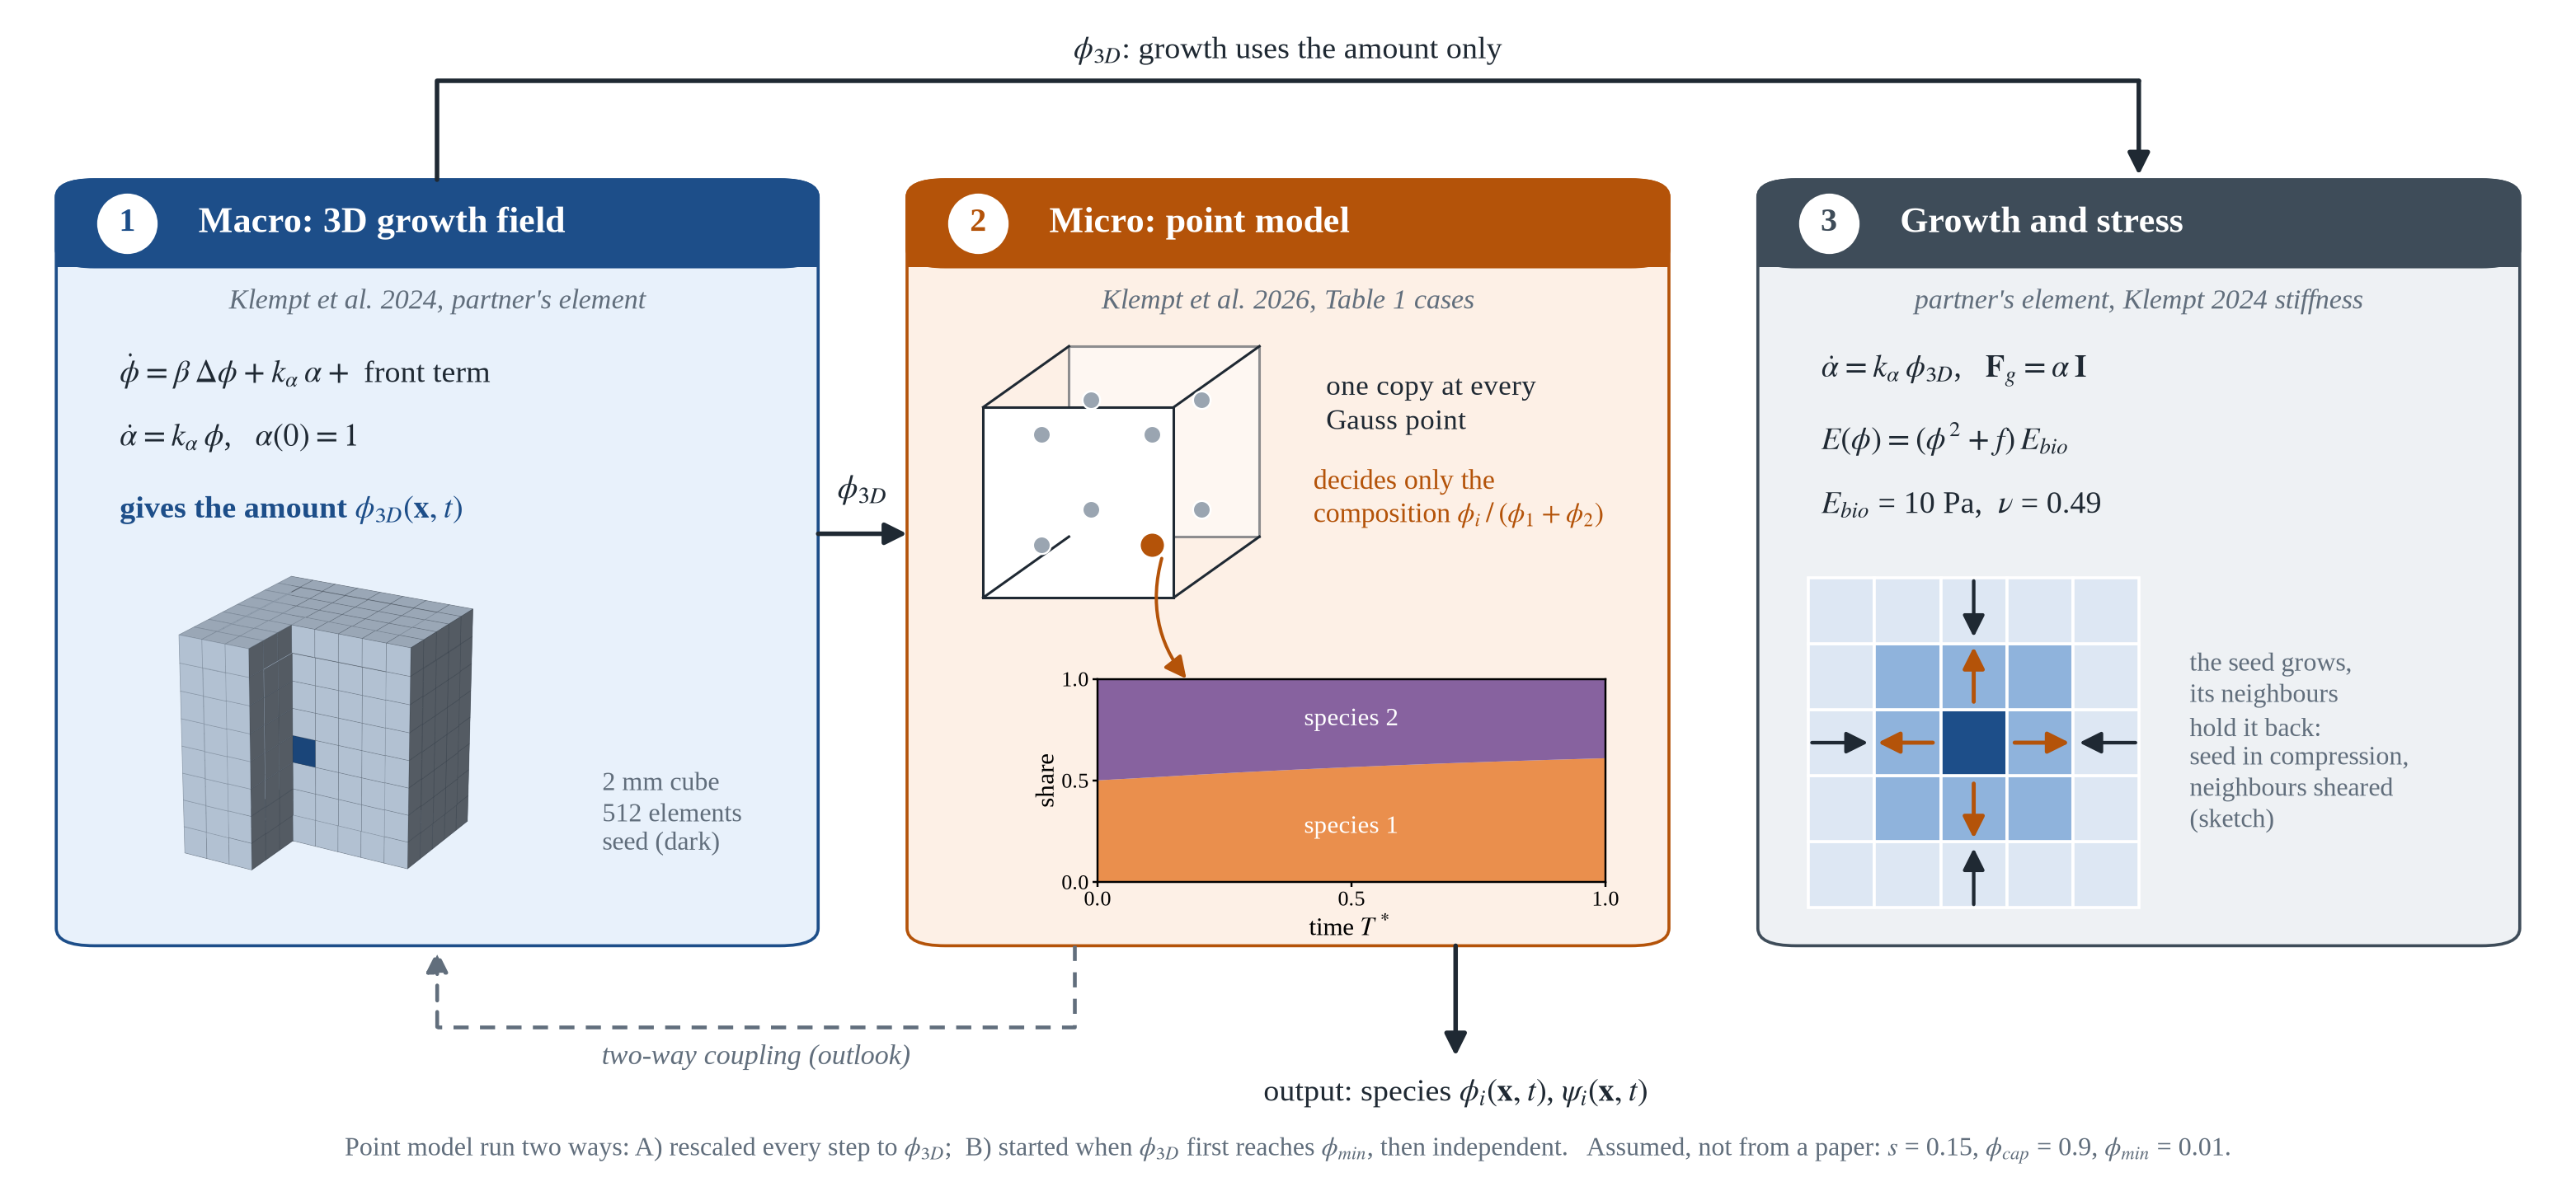
\includegraphics[width=0.80\textwidth]{fig_coupling_schematic.png}
  \caption{\textbf{連成の構成．}
    (1) 成長の場（Klempt 2024）が量 $\phi$ を決め，
    (2) 各 Gauss 点の点モデル（Klempt 2026）が組成を決め，
    (3) 成長と応力は量だけを使う（一方向の連成）．}
  \label{fig:coupling}
\end{figure*}

\subsection{検証}

材料ルーチンは閉じた形の解（拘束成長，自由成長）を丸め誤差の範囲で再現した．
ANSYS の中の連成計算は，勾配のない領域の厳密解に $\alpha$ で $3\times10^{-11}$ まで一致した．
2 菌種の計算では，ANSYS から点モデルへのすべての呼び出しを Python で同じ値に再現し，
論文に示された結果（共存，一方の菌種の勝ち残り）が保たれることを確かめた．

\subsection{拡散係数とメッシュ収束}

$\phi$ の拡散係数 $\beta$ は，Klempt 2024 の Table\,2 の値を 2\,mm の立方体に換算した
$\beta=0.02$\,mm$^2/T^*$ を用いた（換算は仮定である）．
陽解法の安定条件 $h^2/(2\Delta t)\ge\beta$\cite{rudolf2025} は全メッシュで満たされる．
表\,\ref{tab:mesh} に示すとおり，シードの平均応力と周囲の引張りは
$8^3$，$16^3$，$24^3$ の要素で 3\% 以内に一致した．
要素の入力例の値 $\beta=10^{-4}$ では拡散の長さが要素より小さく，応力は収束しない．

\begin{table}[tb]
  \begin{center}
    \caption{ANSYS でのメッシュ収束（$T^*=1.1$，$E=10$\,Pa，単位 Pa）}
    \vspace{2mm}
    {\small
    \begin{tabular}{lccc}\hline
       & $8^3$ & $16^3$ & $24^3$ \\\hline
      シード平均応力 [$10^{-4}$] & $-2.52$ & $-2.53$ & $-2.45$ \\
      周囲 1 層の引張り [$10^{-5}$] & $6.01$ & $6.04$ & $5.85$ \\
      シード von Mises [$10^{-4}$] & $4.83$ & $5.87$ & $6.06$ \\\hline
    \end{tabular}
    }
    \label{tab:mesh}
  \end{center}
\end{table}

\subsection{2 菌種の組成}

2 菌種の組成は，結合時間 $s$，時間 $T^*$，局所の栄養 $c_{\rm rel}$ の積
$s\,T^*c_{\rm rel}$ だけで決まった（図\,\ref{fig:clock}）．
栄養が点モデルの時計の役割をする．
一方の菌種が勝つ場合（Klempt 2026 のケース 6）は，
$s\,T^*c\approx0.03$ から $0.08$ の間で入れ替わりが起こり，
結果は初期の割合が約 0.51 を境に分かれる（双安定）．

\begin{figure}[tb]
  \centering
  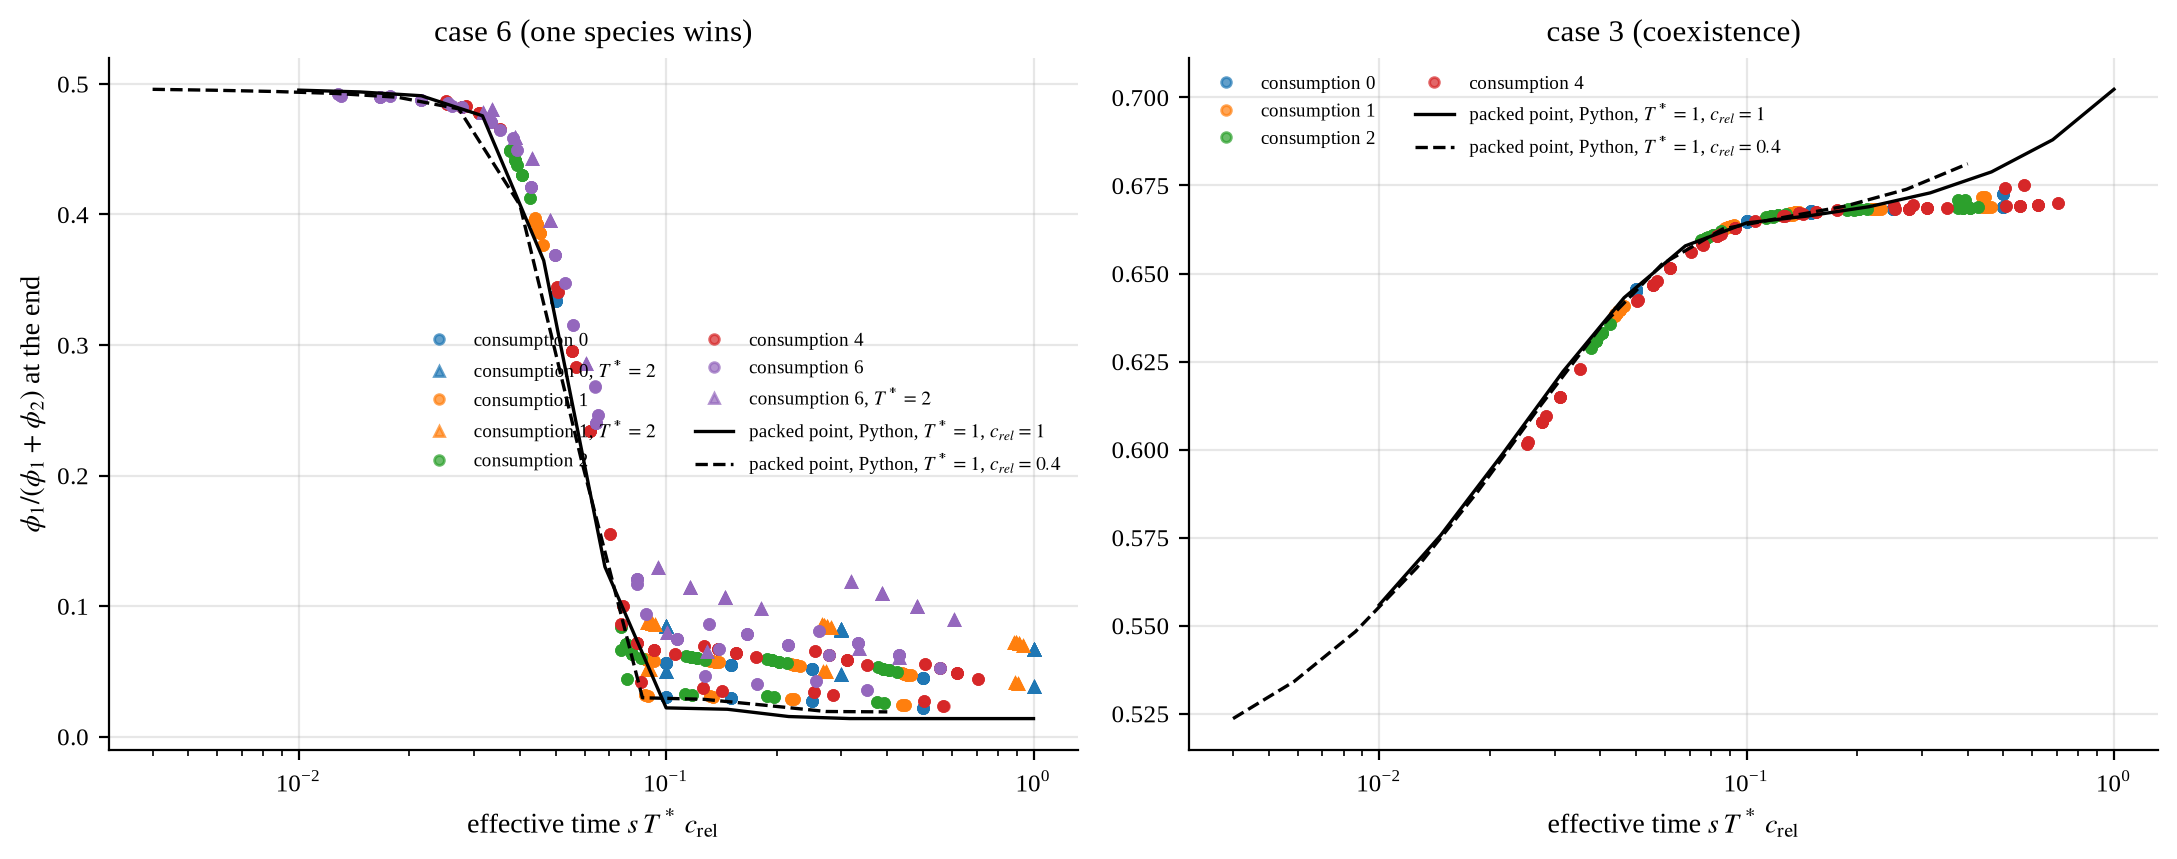
\includegraphics[width=\linewidth]{fig_composition_clock.png}
  \caption{\textbf{組成の「時計」．} ANSYS の全シード要素の終状態の割合を
    $s\,T^*c_{\rm rel}$ に対して描くと，1 本の曲線に乗る（線は Python の点モデル）．}
  \label{fig:clock}
\end{figure}

%%=================================================================
\section{考察}
%%=================================================================

\subsection{Hamilton 原理による対称性の利点}

$\mathbf{A}$ の対称性は自由エネルギーの二次形式から自動的に従う．
非対称を仮定すると推定するパラメータは 25 個となり，各条件の観測 25 個に対して識別できない．
対称性により，推定できる 15 次元の問題になる．

\subsection{Dysbiotic 条件での相互作用の変化}

DH では \textit{Fn}--\textit{Pg} と \textit{Vei}--\textit{Pg} の正の成分が強く現れた
（$\hat a_{45}=5.63$，$\hat a_{55}=3.43$，DS ではそれぞれ 2.20，0.30）．
共生条件ではこれらの成分は事後分布でゼロに集中し，固定しなくても推定から現れた．
\textit{Pg} の株の違い（共生条件 DSM\,20709，疾患型条件 W83）は，
本モデルでは \textit{Pg} に関わる成分の違いとして吸収される．

\subsection{限界と慶應での展開}

連成は一方向であり，組成も応力も場に戻らない．
また検証（verification）は行ったが，実験との比較（validation）は行っていない．
$\beta$ は換算した仮定の値であり，応力の大きさは弾性率に比例する．

慶應では，(1) Klempt 2024 の Eq.\,30 にある力学の項を戻す「応力から成長へ」の連成と，
(2) 同じ問題を ANSYS（NEM，陽解法）と Abaqus（通常の有限要素，陰解法）で解く数値面の比較を中心に続ける．
Abaqus 版は $48^3$ までメッシュ収束を確かめ，点モデルを Fortran に移して 4--9 倍速くした．

%%=================================================================
\section{結論}
%%=================================================================

拡張 Hamilton 原理に基づく多菌種の点モデルと成長の場のモデルを，
推定と有限要素解析の両面から結び付けた．主な成果を以下に示す．

\begin{enumerate}
  \item 5 菌種の相互作用 15 成分を 2 段階 GPU-TMCMC で推定した．
        GPU で CPU の約 200 倍の速さとなり，
        推定に使っていない pH を $R^2=0.778$ で予測した．
  \item 成長の運動学 $\mathbf F_g=\alpha\mathbf I$ を ANSYS の材料ルーチンとして実装し，
        閉じた形の解と厳密解で検証して，バイオフィルムの有限要素に組み込んだ．
  \item 2 菌種について，場が量を，点モデルが組成を決める連成を行い，
        組成が $s\,T^*c_{\rm rel}$ だけで決まること，ケース 6 が双安定であることを示した．
  \item 換算した $\beta=0.02$\,mm$^2/T^*$ で，シードの応力は $8^3$--$24^3$ で 3\% 以内に収束した．
\end{enumerate}

\paragraph{謝辞}
本研究は LUH 連続体力学研究所での修士論文の一部であり，
Philipp Junker 教授，Meisam Soleimani 博士，Hendrik Geisler 博士の指導を受けた．
実験データは Nils Heine 氏ほか（NIFE/MHH）から提供いただいた．
ここに感謝の意を表する．

\bibliographystyle{custom-unsrt}
\bibliography{reference}
\lastpagesettings

\end{document}

\lastpagecontrol{7.0 cm}
